\section{Mon, Aug 27, 2018}

Today doesn't feel like a Monday at all. It feels ... I don't know what it feels
like to be honest. It just feels like a day. A day where the zombies come out and
everyone tends to just do their thing and go around being, well, zombies. I'm sure
the day will improve somehow. Too much going on over the weekend, couldn't fully rest
and relax like I wanted to. Oh well, that's what life does at times I suppose. It
happens to the best of us, or the worst of us. It just happens okay? Okay!

Bought a bunch of used church books. Oh the things that were said in them back in the
day? Talk about some good times for sure. Here's an example about polygamy:

\begin{figure}[h!]
  \centering
  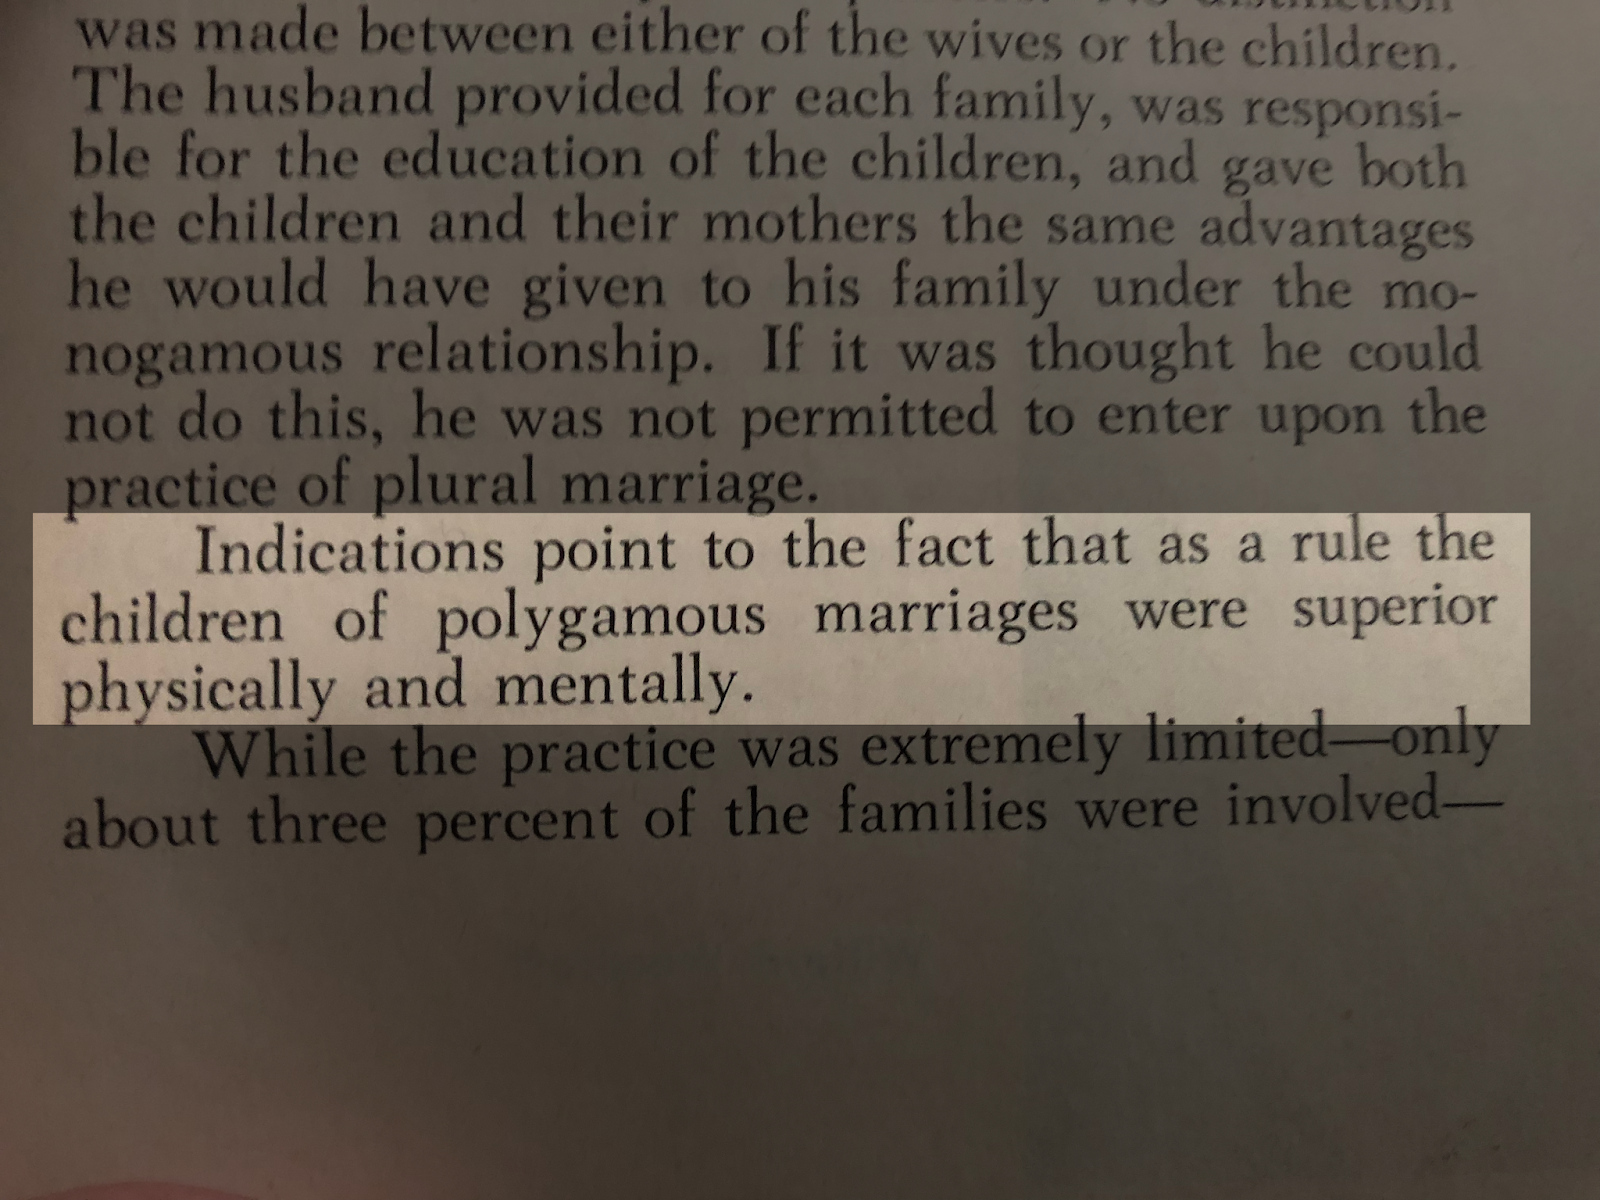
\includegraphics[width=1\linewidth]{2018/images/polygamy.png}
  \caption{What of the Mormons? Gordon B. Hinckley, page 203}
  \label{fig:polygamy}
\end{figure}

Sometimes I don't know what to think about what they were up to or thinking. I
honestly haven't the slightest idea. But well, those were different times I guess. If
that's even a valid excuse for anything which they have said.

Now if I could just wake up. This whole getting up at 6:30 am thing is really not for
me. I mean it could be for me, but it's not. That's how wonderful life is at times.
That's just simply how great and awesome and amazing everything tends to turn out.
But I digress. There needs to be something that can just wake me up, and get the cats
out of my room so I don't end up locking them in there. Ha!\footnote{Yeah, it's 
happened on a few occasions, the cat just sits on the bed waiting for me to get home
and then I open the door and he stares me down like, seriously? Do you know how long
I was in there? But he's purring and happy so I guess that's a win right?}

\st{I kinda want this life to simply be over. It would be nice if I could end it all,
find a way to just make it go away. People would be sad though, and who would take
care of things while I was gone etc? It wouldn't be fair to those around me, so I 
can't. What a selfish thought to have.}

This week should be bright and full of hope, at least I hope it will be. If it's not?
Well then there's something wrong with it all and we just don't know what will happen
at that point now will we. No, I didn't think so. Man it feels like I tend to ramble
a bit in these entries. Is that the case? Should I dial it back? Oh you don't know do
you. You're just reading this. Shoot.

\subsection{9:14 AM}

One would think I would be able to get past all of these thoughts by now. So many
thoughts come and go into my mind that I simply cannot contain them all. Yeah it
would be very nice to simply be able to get by without any of them. Stupid thoughts
need to go away. But they don't, and here \st{we are} I am. There is no we in I,
that's all there is to this life. I am but a single person alone on this island known
as life. Whatever is to be had of me, let it be. I will bear my afflictions alone.

\subsection{10:00 AM}

If there is a God, and He is out there looking over His creations, one has to wonder
at times how far will He allow people to suffer. We are told that God allows
suffering to happen because it's all part of experiencing this life and learning from
our actions, aka agency. We have agency. Sometimes we make mistakes and that causes
our suffering. This is not always the case, sometimes suffering just happens to good
and bad people for no fault of their own. Again, it's all about being able to have
experiences in this life.

I have a hard time with this thought. With so many people on this earth going through
an experience, and the conditions that some people live in and are born in etc. It
doesn't feel fair. People have used scripture\footnote{Acts 17:26-27} to dictate how 
all of this comes about, but still I don't see it.